\documentclass{beamer}
\newcommand{\myfont}{\rmfamily\normalsize\upshape\mdseries}
\newcommand{\degree}{^\circ}
\title{\sffamily Review II(Slides 72 - 116)}
\subtitle{\textbf{Logics \& Induction }\\ Start from the very begining...}
\institute[UM-SJTU JI]{University of Michigan-Shanghai Jiao Tong University Joint Institute}
\author{HamHam}
\usepackage{graphicx}
\usepackage{picinpar}
\usepackage{indentfirst}
\usepackage{chemformula}
\usepackage{geometry}
\usepackage{subfigure}
\usepackage{appendix}
\usepackage{amsfonts,amsmath,amssymb}
\usepackage{bm,bbm}
\usepackage{enumerate}
\usepackage{float}
\usepackage{geometry}
\usepackage{latexsym}
\usepackage{multicol,multirow,multido}
\usepackage{tabularx}
\usepackage{ulem}
\usepackage{tikz}
\usepackage{color,xcolor}
\usepackage{cite}
\usepackage{setspace}
\usepackage{hyperref}
\usepackage{textpos}
\usepackage{booktabs}
\usepackage{diagbox}
\usepackage{listings}
\usepackage{minted}
\usepackage{JI_MathCourse_Notations}
\usetheme[dove]{Boadilla}
\usecolortheme{dolphin}
%\pgfdeclaremask{figmask}{or_circuit.jpg}
%\pgfdeclareimage[mask=figmask,width=0.6\textwidth]{or_circuit}{or_circuit_1.png}
\useoutertheme{miniframes}
\begin{document}
    \usebackgroundtemplate{\tikz\node[opacity=0.25]{
    
\includegraphics[width=\paperwidth,
    height=\paperheight]{hamster.jpg}
    };}
\begin{titlepage}
    \begin{center}
        VE203 - Discrete Mathmatics 
    \end{center}
\end{titlepage}
\myfont
\section{Logics}
\begin{frame}
    \frametitle{Summary}
    \begin{itemize}
        \item Sets
        \begin{itemize}
            \item * Definitions \& Operations
            \item Application: Graph
        \end{itemize}
        \item Logics
        \begin{itemize}
            \item Logical Variable \& Operations
            \item Concepts: Vacuous truth, Tautology, Predicate, Quantifier$\dots$
            \item * Predicate Logic (First-Order Logic): Truth Tree
            \item * Propositional Logic: Natural Deduction Tree
        \end{itemize}
        \item Induction
        \begin{itemize}
            \item * Weak/Strong(Complete) Induction (Type I/II Induction)
            \item Structual Induction
            \item Correctness of Sorting Algorithms
            \item Concepts: WOP, Monoid
        \end{itemize}
    \end{itemize}
\end{frame}
\begin{frame}
    \frametitle{Updates}
    \begin{enumerate}
        \item Textbook: Galliar
        \item Some Typo Fixed
        \item Format of Truth-Tree Proof
    \end{enumerate}

\end{frame}
\begin{frame}
    \frametitle{Natural Deduction Tree}
    \Large{
    \begin{block}{{\Large General Rule}}
        $$\frac{\text{given that}\dots}{\text{we conclude that}\dots} \text{What was done}$$
    \end{block}
    }
    \Large{
        \begin{block}{{\Large Strategy}}
            \begin{enumerate}
                \item Introduction: We want more!
                \item Elimination: We want less!
            \end{enumerate}
        \end{block}
    }
    Reference: \url{https://www.youtube.com/watch?v=v-1ikd_89Mg}
\end{frame}
\begin{frame}
    \frametitle{Natural Deduction Tree}
    \begin{table}[htbp]
        \begin{tabular}{|p{3mm}|>{\centering\arraybackslash}p{4.5cm}|>{\centering\arraybackslash}p{4.5cm}|}
        \toprule
        & Introduction & Elimination \\
        \midrule
        \rule{0pt}{0.6em} $\wedge$ &  & \\
        \rule{0pt}{0.6em} &  & \\
        \rule{0pt}{0.6em} $\vee$ &  & \\
        \rule{0pt}{0.6em} &  & \\
        \rule{0pt}{0.6em} $\rightarrow$ &  & \\
        \rule{0pt}{0.6em} &  & \\
        \rule{0pt}{0.6em} $\neg$ &  & \\
        \rule{0pt}{0.6em} &  & \\
        \bottomrule
        \end{tabular}
    \end{table}
\end{frame}
\begin{frame}
    \frametitle{Introduction on False / Negation}
    \centering
    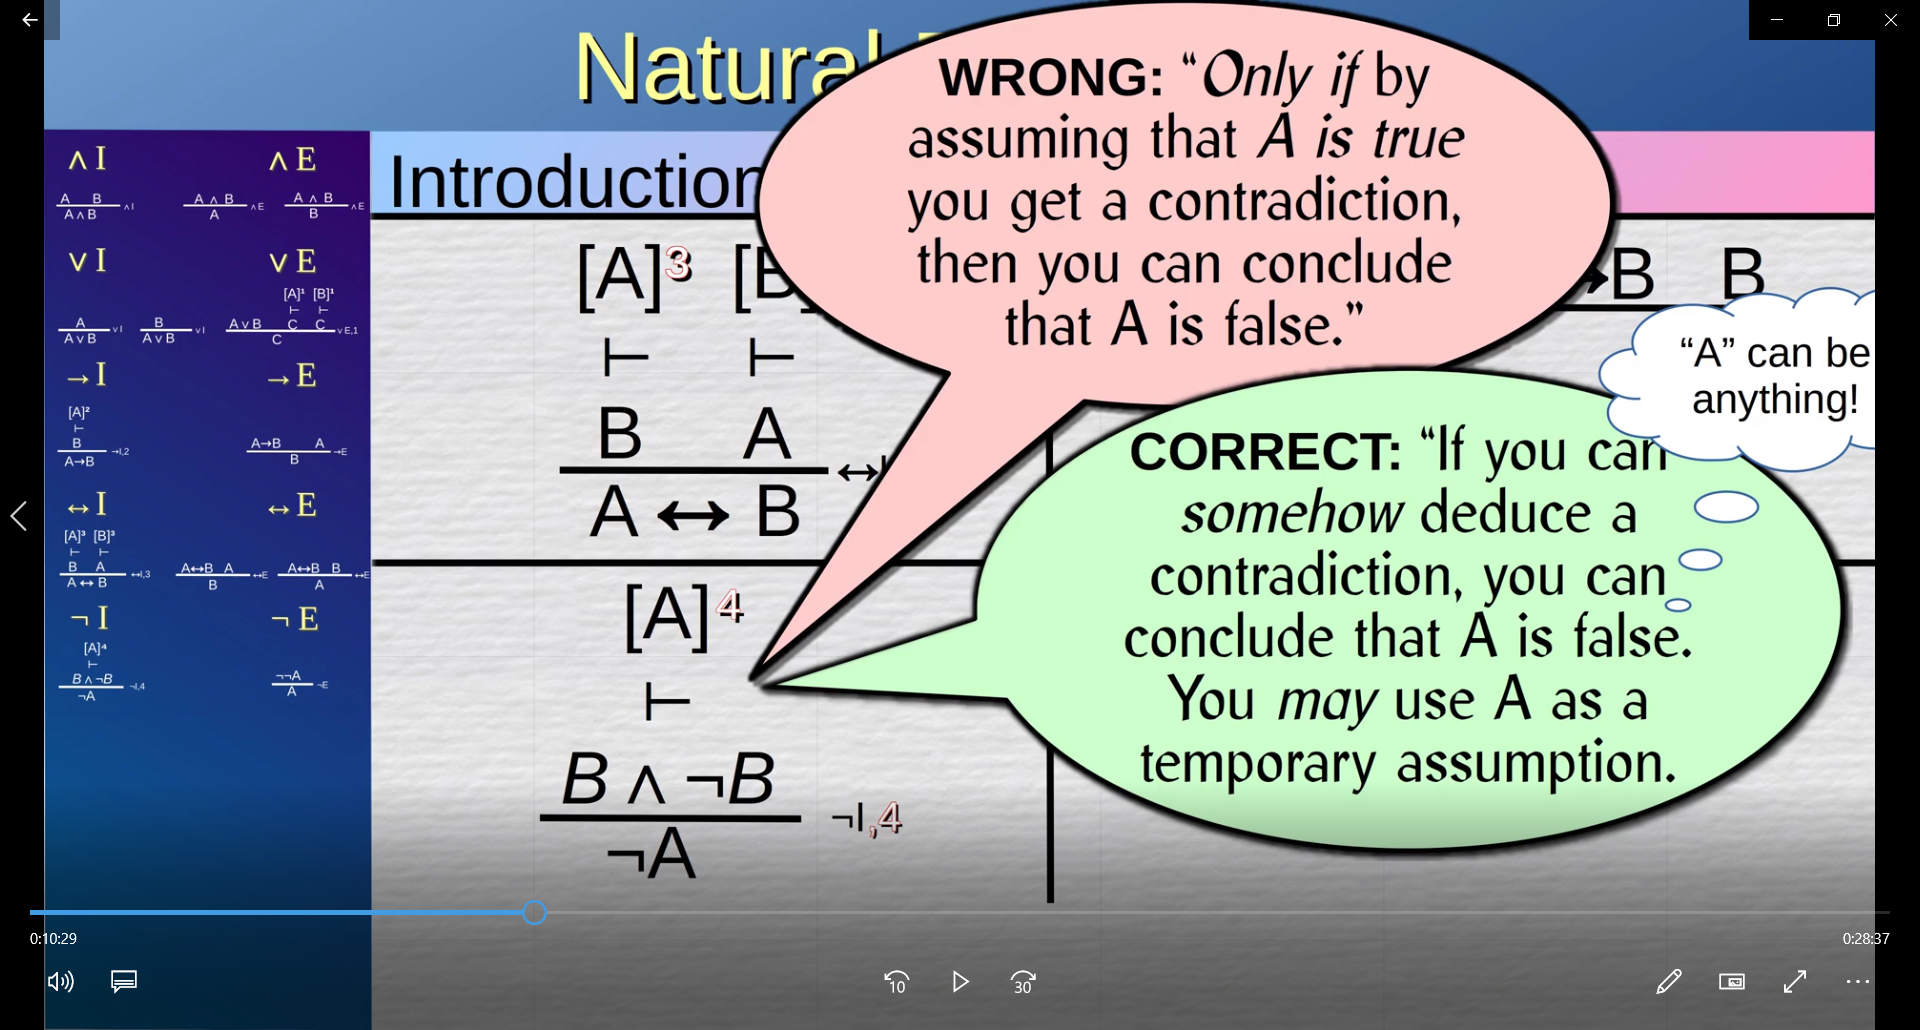
\includegraphics[width=0.9\textwidth]{elimination.png}
    
\end{frame}
\begin{frame}[fragile]
    \frametitle{Exercise}
    1. Use Natural Deduction Tree to prove
    \begin{enumerate}
        \item $(X \wedge Y\, ) \vee (Z \wedge Y\, ) \vdash Y$
        \item $\neg A, A\vee B \vdash B \vee C$
    \end{enumerate}
    \vspace{2em}
    \pause
    \begin{minipage}[b]{0.43\linewidth}
        \centering
        \fbox{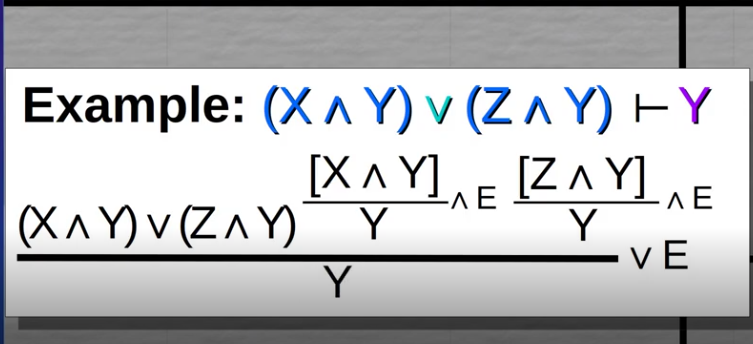
\includegraphics[width=1\linewidth]{ans1.png}}
    \end{minipage}
    \begin{minipage}[b]{0.43\linewidth}
        \centering
        \fbox{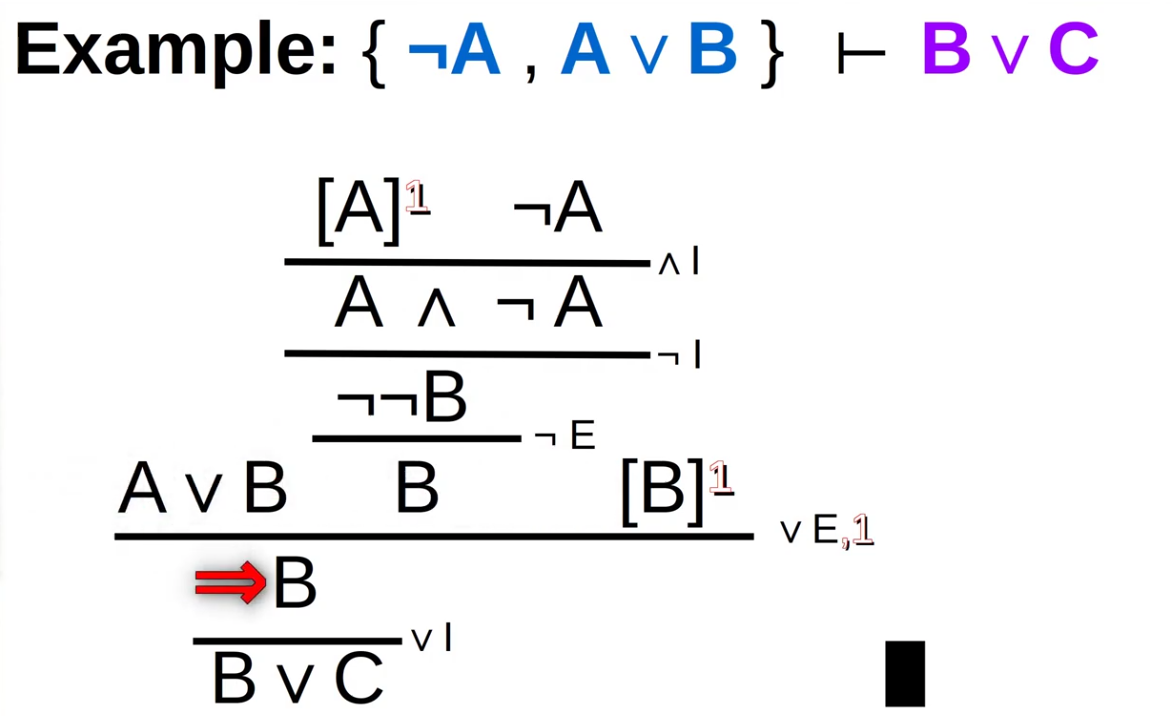
\includegraphics[width=1\linewidth]{ans2.png}}
    \end{minipage}
\end{frame}
\section{Induction}
\begin{frame}
    \frametitle{Mathematical Induction}
    \begin{block}{Weak Induction (Type I Induction)}

        Supppse over $\mathbb{N}$ we have
        \begin{enumerate}
            \item $P(k)$
            \item $\forall n \geq k, \quad P(n) \rightarrow P(n+1)$
        \end{enumerate}
    
        Then $\forall n \geq k, \quad P(n)$. Usually we have $k=0$ as base case.
    \end{block}
    
    \begin{block}{Strong(Complete) Induction (Type II Induction)}
        \begin{enumerate}
            \item $P(0)$
            \item $\forall n \geq 1, \quad [P(0) \wedge P(1)\wedge \dots \wedge P(n-1) \rightarrow P(n)]$
        \end{enumerate}
        Then $\forall n, \quad P(n)$.
    \end{block}
    

\end{frame}

\begin{frame}[fragile]
    \frametitle{Mathematical Induction}

    \begin{minipage}[b]{0.60\textwidth}
        \small
        \begin{itemize}
            \item \textbf{Weak induction} is like a line of dominoes where each domino
            \red{only depends on the one immediately before it}. The proof establishes that if the first domino falls, 
            it will topple the next one, which, in turn, knocks down the subsequent one. 
            By this chain reaction, the entire row of dominoes falls.
            \item \textbf{Strong induction} is like a line of dominoes where each domino has the ability 
            to \red{knock down all the dominoes that come after it}. 
            By assuming that when any domino falls, it has a cascading effect on all 
            the dominoes ahead, the proof establishes that if the first domino falls, 
            it will eventually cause the entire row of dominoes to collapse.
        \end{itemize}
    \end{minipage}
    \hspace{-2mm}
    \begin{minipage}[b]{0.32\textwidth}
        \begin{figure}
            \centering
            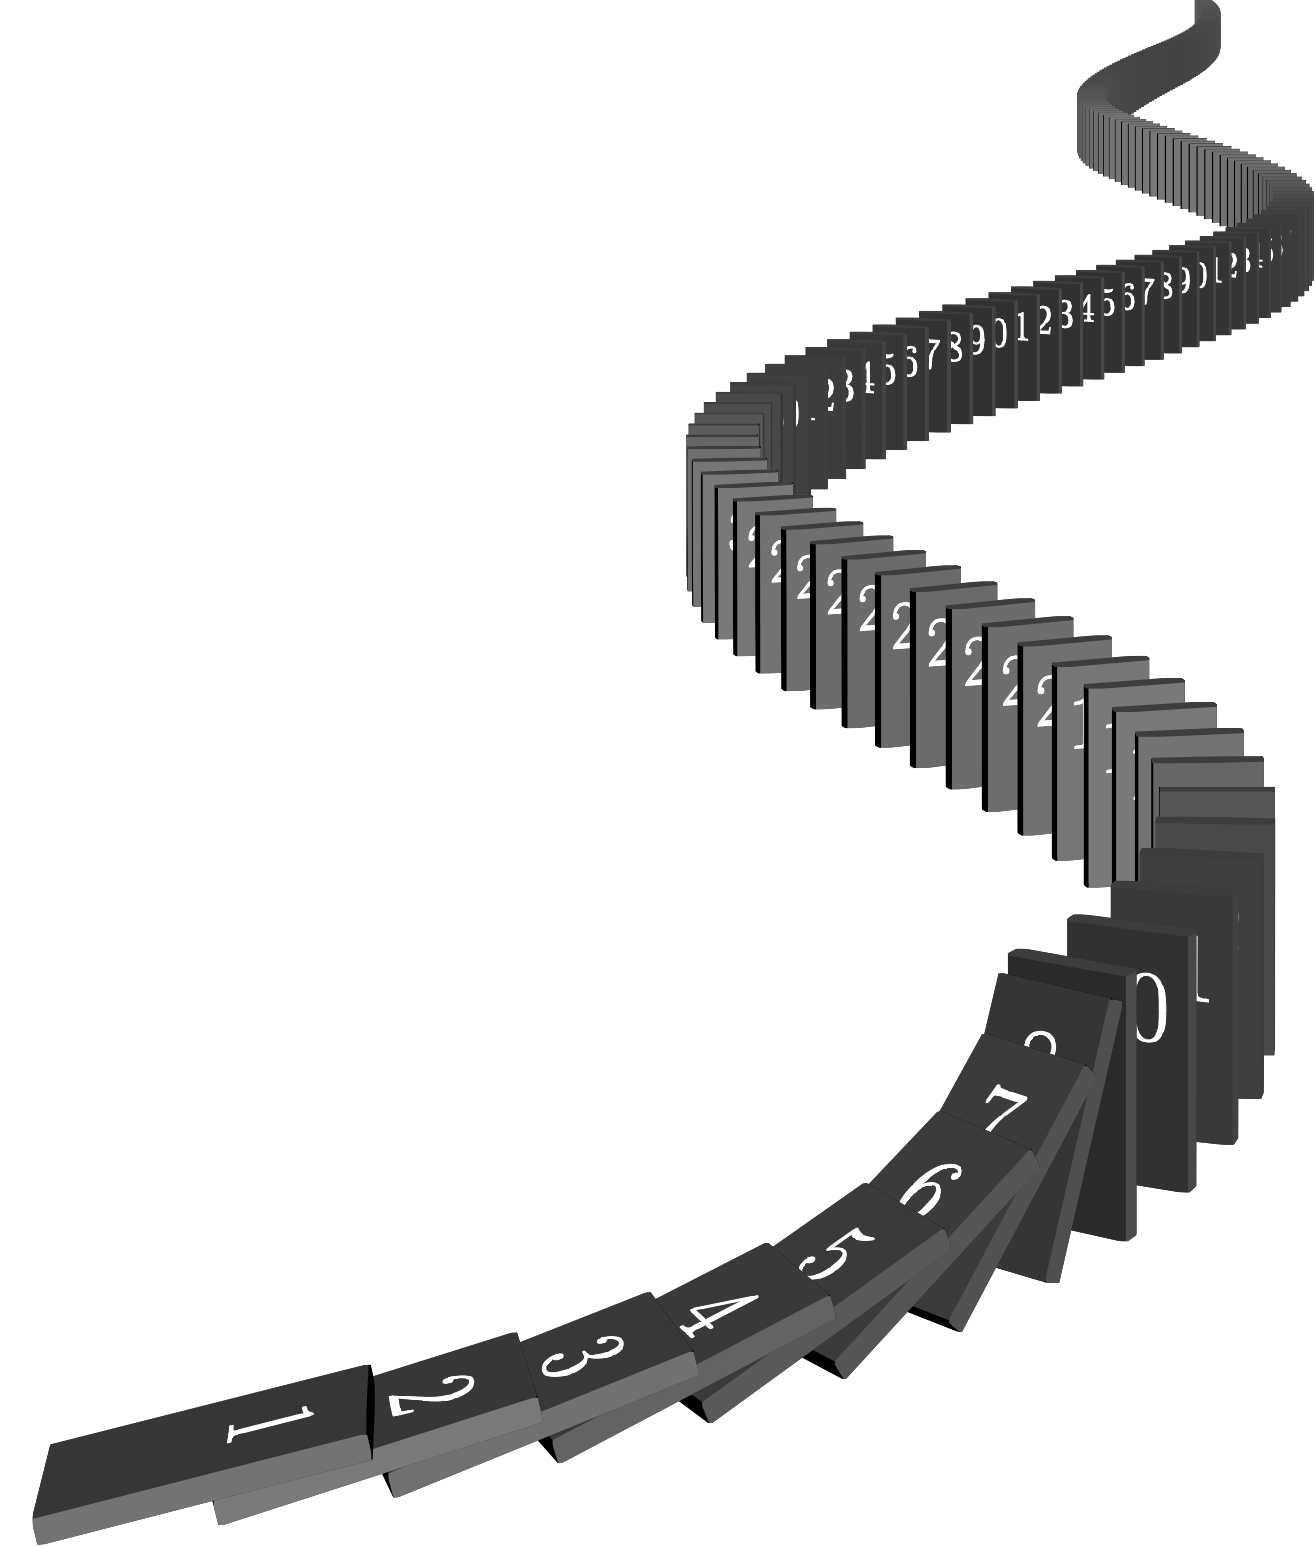
\includegraphics[width=1\textwidth]{domino.png}
            \caption{Falling dominoes}
        \end{figure}

        \vspace{2em}

    \end{minipage}

\end{frame}
\begin{frame}
    \frametitle{Induction ``Paradox" (Slides 93)}

    For any $n \in \mathbb{N} \cut \{0\}$, there exist integers $a_n$ and $b_n$ s.t.
    $$
    \(\frac{1+\sqrt{5}}{2}\)^n = \frac{a_n+b_n \sqrt{5}}{2}
    $$

    \begin{enumerate}
        \item Base case: $n=1$, clear by taking $a_1=b_1=1$
        \item Inductive case: assume the IH for $n\geq 1$,
        \begin{equation*}
        \begin{aligned}
            \(\frac{1+\sqrt{5}}{2}\)^{n+1} & = \frac{a_n + b_n \sqrt{5}}{2} \cdot \frac{1+\sqrt{5}}{2}\\
            & = \frac{(a_n+5b_n)/2 + ((a_n+b_n)/2) \sqrt{5}}{2}
        \end{aligned}
        \end{equation*}

    \end{enumerate}
\end{frame}
\begin{frame}[fragile]
    \frametitle{Induction ``Example"¿}
    \begin{figure}
        \centering
        \fbox{\includegraphics[width=0.7\textwidth]{ve203_main_horst_cut_119.pdf}}
    \end{figure}
\end{frame}
\begin{frame}
    \frametitle{Induction ``Example"¿}
    \hspace{1em}
    \begin{figure}
        \centering
        \fbox{\includegraphics[width=0.7\textwidth]{ve203_main_horst_cut_120.pdf}}
    \end{figure}
\end{frame}
\begin{frame}
    \frametitle{Exercise}
    
    \begin{figure}
        \centering
        \fbox{\includegraphics[width=0.7\textwidth]{ve203_main_horst_cut_117.pdf}}
    \end{figure}

\end{frame}
\begin{frame}
    \frametitle{Solution}
    
    \begin{figure}
        \centering
        \fbox{\includegraphics[width=0.7\textwidth]{ve203_main_horst_cut_118.pdf}}
    \end{figure}

\end{frame}
\begin{frame}
    \frametitle{Exercise (DIY)}
    2. Let $ a_n$ be the following expression with $n$ nested radicals:\
    $$a_n=\sqrt{2+\sqrt{2+\cdots+\sqrt{2+\sqrt{2}}}}$$
    Please find the explict formula for $a_n$.
\end{frame}
\begin{frame}
    \frametitle{Solution}
    \hh Note that $a_n$ can be defined recursively like this: $a_1 =\sqrt{2}$, and
    $a_{n+1} =\sqrt{a_n+2}$ for $n \geq 1$. We proceed by induction. \\
    \red{Hypothesis:} $a_n= 2 \cos \frac{\pi}{2^{n+1}}$\\
    \red{Base case:} $a_1=\sqrt{2}$, and $2\cdot \cos \frac{\pi}{4}= 2\cdot \frac{1}{\sqrt{2}}=\sqrt{2}$.\\ 
    \red{Inductive case:} assuming the \textbf{\red{IH}} is true for n, then 
    {
    \small
    \begin{equation*}
    \begin{aligned}
        a_{n+1}&=\sqrt{2+a_n}=\sqrt{2+2\cos \frac{\pi}{2^{n+1}}}\\
               &=\sqrt{2+2\cos \frac{2\pi}{2^{n+2}}}\\
               &=\sqrt{2+2(2\cos^2\frac{\pi}{2^{n+2}}-1)}\\
               &=\sqrt{4\cos ^2\frac{\pi}{2^{n+2}}}
               =2\cos \frac{\pi}{2^{n+2}}
    \end{aligned}
    \end{equation*}
    }
    By  induction, we conclude that $a_n = 2 \cos \frac{\pi}{2^{n+1}}$.
\end{frame}


\section{*Extra Topic}
\begin{frame}
    \frametitle{Sorting Algorithms}
    We have lots lots of sorting algorithms!
    \vv
    \begin{itemize}
        \item Demostration: \url{https://www.sortvisualizer.com/quicksort/}
        \item Classification
        \item Costs
                \begin{itemize}
                    \item Time complexity (Worst/Averge/Best)
                    \item Space complexity
                    \item Stability
                \end{itemize}
    \end{itemize}
    \begin{block}{Question}
        \hh How to choose a sorting algorithms that most satisfy your need?
    \end{block}
\end{frame}


\begin{frame}[fragile]
    \frametitle{Quick Sort with Second key word}

    \begin{minted}[mathescape,linenos,numbersep=2pt,
            gobble=2,frame=lines, fontsize=\small]{cpp}
  void QuickSort(vector<int>& v, vector<int>& o,
                 int left, int right){
      if (left>=right)  return;
      int key = (left+right)/2;// you can also choose right/left
      while (left<right){
          while (left<right && (v[right] > v[key] || 
            v[right]==v[key] && o[right]>o[key]))  right--;
          while (left<right && (v[left] <= v[key] || 
            v[left]==v[key] && o[left]<o[key]))   left++;  
          if (left < right) swap(v[left], v[right]);   
      }
      swap(v[left], v[key]);   //left== right
      int meet= key;     //divide into two parts
      QuickSort(v, o, left, meet-1); 
      QuickSort(v, o, meet+1, right); 
  }
    \end{minted}

\end{frame}
\begin{frame}[fragile]
    \frametitle{Modified Bubble Sort}
    \begin{minted}[mathescape,linenos,numbersep=2pt,
        gobble=2,frame=lines, fontsize=\footnotesize]{java}
  public static void bubble_sort(int[] intArr) {
      int max = intArr.length - 1;
      int secondCount = max;  //record where the exchange happen last time
      for (int i = 0; i < max; i++) {
          System.out.println( (i + 1) + "times" );
          boolean flag = true;int lastChangeIndex = 0;
          for (int j = 0; j < secondCount; j++) {
              if (intArr[j] > intArr[j + 1]) {
                  swap(Arr[j],Arr[j+1]);
                  flag = false;
                  lastChangeIndex = j;
              }
              System.out.println("Compare:"+(j+1)+", Result:"+Arrays.toString(intArr));
          }
          if (flag) break; //already well ordering
          secondCount = lastChangeIndex; //update
      }
  }
    \end{minted}
\end{frame}
\begin{frame}
    \frametitle{Exercise}
    3. Try to implement \blue{three-way merge sort} in C++.
    If you know \blue{Master Theorem}, try to calculate the time complexity and compare with the 
    original merge sort.
    \vs{4em}\\
    4. Exercise regarding sorting algorithms:
    \begin{itemize}
        \item \url{https://leetcode.cn/problems/insertion-sort-list/}
        \item \url{https://leetcode.cn/problems/kth-largest-element-in-an-array/}
    \end{itemize}
\end{frame}
\begin{frame}
    \frametitle{Reference}

    \begin{itemize}
        \item Lecture Slides from Ve203 FA 2020 by Horst Hohberger.
        \item Examples from Vv286 Lecture Slides.
        \item Exercises from 2021-Fall-Ve203 TA Zhao Jiayuan
        \item Stable Quick Sort, \url{https://blog.csdn.net/liuchenjane/article/details/72902325}
        \item Modified Bubble Sort, \url{https://blog.csdn.net/weixin_43168559/article/details/88873585}
        \item Picture "Falling Dominoes", \url{https://crystalclearmaths.com/videos-learning-resources/iterations-repeating-patterns/mathematical-induction/}
    \end{itemize}

\end{frame}
\end{document}